% Created 2015-11-18 Wed 20:56
\documentclass[presentation]{beamer}
\usepackage[utf8]{inputenc}
\usepackage[T1]{fontenc}
\usepackage{fixltx2e}
\usepackage{graphicx}
\usepackage{longtable}
\usepackage{float}
\usepackage{wrapfig}
\usepackage{rotating}
\usepackage[normalem]{ulem}
\usepackage{amsmath}
\usepackage{textcomp}
\usepackage{marvosym}
\usepackage{wasysym}
\usepackage{amssymb}
\usepackage{hyperref}
\tolerance=1000
\usepackage{color}
\usetheme{default}
\author{Robert W Rankin (Murdoch University, PhD Candidate)}
\date{\today}
\title{Introduction to Bayesian Inference}
\hypersetup{
  pdfkeywords={},
  pdfsubject={},
  pdfcreator={Emacs 24.3.1 (Org mode 8.2.5g)}}
\begin{document}

\maketitle
\begin{frame}{Outline}
\tableofcontents
\end{frame}

\begin{frame}[label=sec-1]{Outline}
\begin{block}{Philosophical differences}
\begin{itemize}
\item Frequentists vs. Bayesian
\end{itemize}
\end{block}

\begin{block}{Priors}
\begin{itemize}
\item densities, impacts
\end{itemize}
\end{block}

\begin{block}{Practise: JAGS}
\end{block}
\begin{block}{Computation (e.g., Gibbs sampling, MCMC; if time)}
\begin{itemize}
\item simulation-based approximatation of the Posteriors
\end{itemize}
\end{block}
\end{frame}
\begin{frame}[label=sec-2]{Advantages of Bayesian Inference}
\begin{itemize}
\item inference statesments: easy to understand (only Bayesians can make probabilistic statements about $\theta$)
\item small sample sizes: exact inference
\item missing data: very easy to impute
\item integrate other information, or calculate 'derived parameters'
\end{itemize}
\begin{block}{Hierarchical Bayesian}
\begin{itemize}
\item model dependences (space \& time)
\item "random-effects" models
\item "model-selection" / "model-multi inference" (AIC, Lasso, etc., are just types of Bayesian models)
\item shrinkage: deflate influence of outlier values
\end{itemize}
\end{block}
\end{frame}
\begin{frame}[label=sec-3]{What is "Bayesian" inference?}
\begin{block}{what comes to mind when you think about "Bayesian"}
\begin{itemize}
\item ???
\end{itemize}
\end{block}
\end{frame}

\begin{frame}[label=sec-4]{What is "Bayesian" inference?}
\begin{block}{what comes to mind when you think about "Bayesian"}
\begin{itemize}
\item Priors: most common ecologist's answer (not necessarily true)
\item Posterior density
 $p(\theta\vert Y)$
\end{itemize}
-- "(posterior) probability density of $\theta$ \emph{given} the observed data $Y$".
\begin{itemize}
\item inference on $\theta$ \emph{given} data
\item $\theta$ has a \textbf{distribution} of values
\end{itemize}
\end{block}
\end{frame}
\begin{frame}[label=sec-5]{What is "Bayesian" inference}
\begin{block}{compare to the Likelihood}
\begin{itemize}
\item Priors
\item Posterior density
 $p(\theta\vert Y)$
\end{itemize}
-- "(posterior) probability density of $\theta$ \emph{given} the observed data $Y$".
-- \emph{Only} Bayesian's have access to the Posterior
\begin{itemize}
\item Likelihood: $p(Y;\theta)$
\end{itemize}
-- "the joint probability of a realization of the data \emph{given} a particular value of $\theta$".
\end{block}

\begin{block}{Maximum-Likelihood}
\begin{itemize}
\item basis most Frequentist analysis
\item Often (but not always) the MLE is the best estimator according to Frequentist's values (consistency, unbiased, etc)
\end{itemize}
\end{block}
\end{frame}

\begin{frame}[label=sec-6]{The likelihood \& Frequentism}
\begin{itemize}
\item before we can talk about the posterior\ldots{} what is the likelihood?
\end{itemize}
\begin{center}
$p(Y \vert \theta)$
\end{center}
\textbf{data} is what is random; $\theta$ is given?
\begin{itemize}
\item find the value of $\theta$ that \emph{maximizes} the probability of having observed the data
\item Frequentist emphasize \emph{repeated use}:
\end{itemize}
if repeat the experiment -> observed slightly different data.  Want estimates that are optimal over all theorectical samples of data.
\end{frame}

\begin{frame}[label=sec-7]{A little demotivation}
\begin{block}{Most Biologists are "Agnostic Bayesians"}
\begin{itemize}
\item \textbf{Frequentist} vs. \textbf{Bayesian}: point estimates nearly identical (under certain conditions)
\end{itemize}
\end{block}

\begin{block}{Example data:}
\begin{itemize}
\item men's height, n=20 observations
\item first run the Frequentist's $\text{glm}(y\sim1)$ function
\end{itemize}
\end{block}
\end{frame}

\begin{frame}[fragile,label=sec-8]{Frequentist Example}
 \begin{block}{Example data:}
\begin{itemize}
\item men's height, n=20 observations
\item first run the Frequentist's $\text{glm}(y\sim1)$ function
\end{itemize}
\color{blue}
\begin{verbatim}
            Estimate Std. Error  t value     Pr(>|t|)
(Intercept) 174.9676   1.530233 114.3405 1.965619e-28
\end{verbatim}

\color{black}
\begin{itemize}
\item Frequentist: start with a point-estimate, then estimate:
\end{itemize}
\color{blue}
\begin{verbatim}
[1] "Frequentist:"
       MLE         se     lo95CI     hi95CI 
174.967636   1.530233 171.968435 177.966837
\end{verbatim}

\color{black}
\end{block}
\end{frame}

\begin{frame}[label=sec-9]{Likelihood}
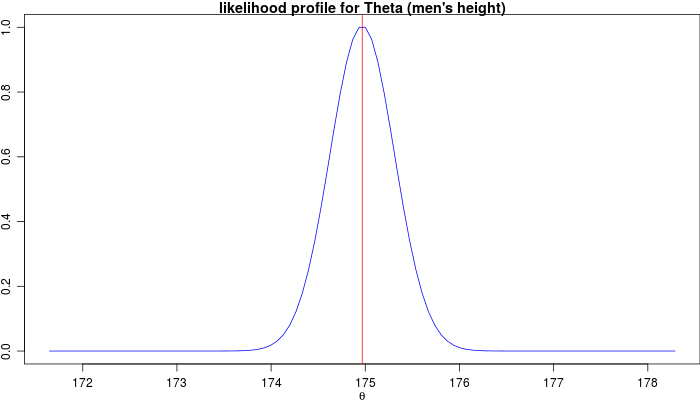
\includegraphics[width=.9\linewidth]{loglike.png}

\begin{itemize}
\item "It would be very (un)likely to have seen the data that I saw, if the value of $\theta$ were X"
\item Choose $\theta$: that which maximize's the likelihood seeing $Y$
\item $\theta_\text{MLE}$ is NOT the "most probabilty value of $\theta$
\end{itemize}
\end{frame}
\begin{frame}[fragile,label=sec-10]{Bayesians: The Posterior}
 \begin{itemize}
\item Frequentist: start with a point-estimate (MLE), then estimate
S.E., 95\% Confidence interval, etc
\end{itemize}
\color{blue}
\begin{verbatim}
[1] "Frequentist:"
       MLE         se     lo95CI     hi95CI 
174.967636   1.530233 171.968435 177.966837
\end{verbatim}

\color{black}
\begin{itemize}
\item Bayesian start with a distribution, and then summarize it with simple descriptive statistics
\end{itemize}
Mean, mode, S.E., 95\% Credibility interval
\color{blue}
\begin{verbatim}
[1] "Bayesian"
       mu        se    lo95CI    hi95CI 
174.83200   1.54682 171.75725 177.91146
\end{verbatim}
\end{frame}
\begin{frame}[label=sec-11]{Posterior density}
\begin{itemize}
\item IS a probability distribution
\end{itemize}
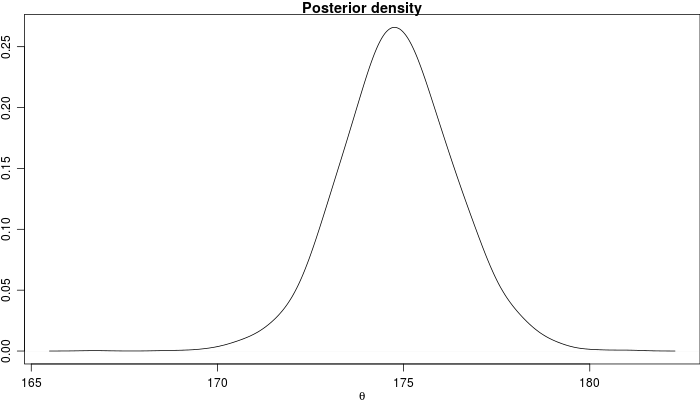
\includegraphics[width=.9\linewidth]{posterior1.png}

\begin{itemize}
\item easy to interpret
\end{itemize}
\end{frame}

\begin{frame}[label=sec-12]{Posterior density}
\begin{itemize}
\item IS a probability distribution
\end{itemize}
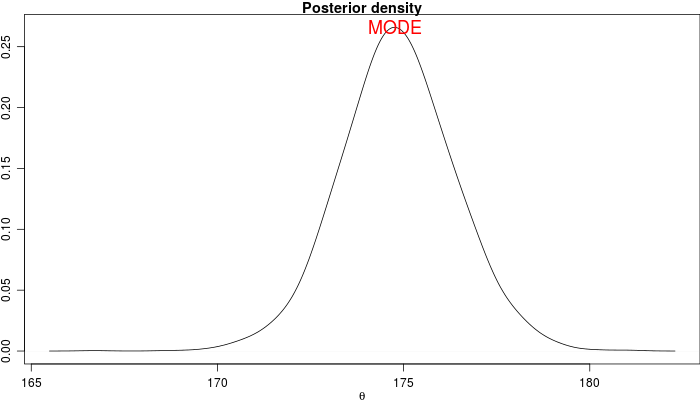
\includegraphics[width=.9\linewidth]{posterior2.png}

\begin{itemize}
\item Posterior mode: most probable value
\item Posterior mean $\mathbb{E}[\theta]=\int p(\theta\vert Y)\theta d\theta$: expected value
\end{itemize}
\end{frame}

\begin{frame}[label=sec-13]{Posterior density}
\begin{itemize}
\item IS a probability distribution
\end{itemize}
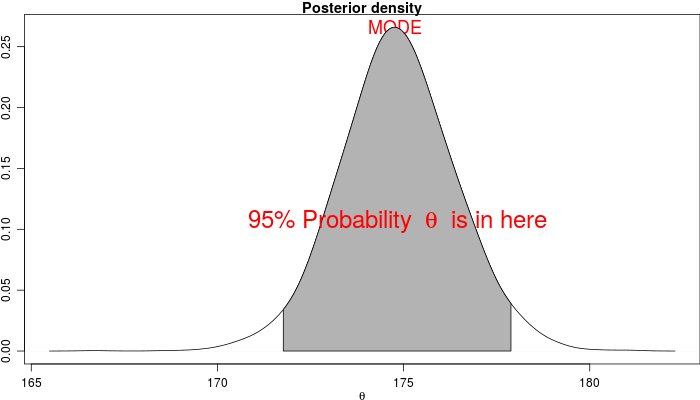
\includegraphics[width=.9\linewidth]{posterior3.png}

\begin{itemize}
\item Posterior mode: most probable value
\item Posterior mean $\mathbb{E}[\theta]=\int p(\theta\vert Y)\theta d\theta$: expected value
\item 95\%CI of $\theta$
\end{itemize}
\end{frame}
\begin{frame}[label=sec-14]{Posterior density}
\begin{itemize}
\item IS a probability distribution
\end{itemize}
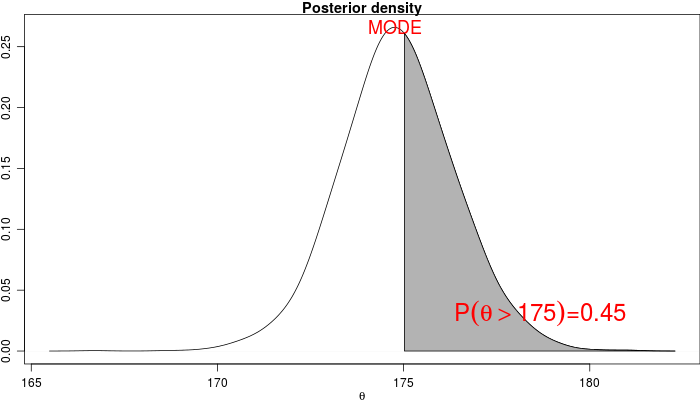
\includegraphics[width=.9\linewidth]{posterior4.png}

\begin{itemize}
\item Posterior mode: most probable value
\item Posterior mean $\mathbb{E}[\theta]=\int p(\theta\vert Y)\theta d\theta$: expected value
\item What is the probability that $\theta>X$? Area of $p(\theta\vert Y)>X$
\end{itemize}
\end{frame}
\begin{frame}[fragile,label=sec-15]{A little demotivation}
 \begin{block}{Most Biologists are "Agnostic Bayesians"}
\begin{itemize}
\item \textbf{Frequentist} vs. \textbf{Bayesian}: point estimates nearly identical (under certain conditions)
\end{itemize}
\color{red}
\begin{block}{Example:}
\begin{itemize}
\item men's height, n=20 observations
S.E. and 95\% CI
\end{itemize}
\color{blue}
\begin{verbatim}
[1] "Frequentist:"
       MLE         se     lo95CI     hi95CI 
174.967636   1.530233 171.968435 177.966837
[1] "Bayesian"
       mu        se    lo95CI    hi95CI 
174.83200   1.54682 171.75725 177.91146
\end{verbatim}

\color{black}
\end{block}
\end{block}
\end{frame}

\begin{frame}[label=sec-16]{A little demotivation}
\begin{block}{Most Biologists are "Agnostic Bayesians"}
\begin{itemize}
\item \textbf{Frequentist} vs. \textbf{Bayesian}: often nearly identical
\item only true for: i) certain "priors", and ii) large-samples sizes
\item key point: \textbf{Be a Master of Priors!}
\end{itemize}
\end{block}
\end{frame}

\begin{frame}[label=sec-17]{Bayesians vs. Frequentism}
\begin{block}{Philosophy}
\begin{itemize}
\item Bayesians: condition on the data, $\theta$ is random
\end{itemize}
think like a gambler
\begin{itemize}
\item Frequentism: data is random
\end{itemize}
think: had we repeated the experiment, we would get different data
\end{block}

\begin{block}{Practical differences?}
mostly, no. BUT, some important situations\ldots{}
\begin{itemize}
\item priors!
\item low-sample sizes, complex models
\item missing data
\item 'optional stopping'
\end{itemize}
\end{block}
\end{frame}

\begin{frame}[label=sec-18]{Posterior Density}
\begin{block}{Posterior: the goal of Bayesian analysis\ldots{}}
\begin{itemize}
\item hard to evaluation
\item Enter \textbf{Baye's Rule}!
\end{itemize}
\begin{center}
$p(\theta\vert Y) = \frac{p(Y\vert \theta)p(\theta)}{\int p(Y\vert \theta)p(\theta) d \theta}$
\end{center}
\end{block}

\begin{block}{Posterior $\propto$ Likelihood x Prior}
\begin{itemize}
\item \emph{likelihood}: easy to evaluate
\item \emph{prior}: express as easy distribution (Norm, Gamma, Beta)
\end{itemize}
\end{block}

\begin{block}{Priors}
defn: "your belief about $\theta$ before observing data", or "a probability distribution about $\theta$ before observing data"
\end{block}
\end{frame}

\begin{frame}[label=sec-19]{Posterior $\propto$ Likelihood x Prior}
\begin{itemize}
\item The posterior: a mixture of "information in the data" (likelihood) and "information in the prior"
\item \textbf{be a master or priors}
\end{itemize}
It is your responsibility to study and know how to express prior information in probabilitistic terms
\end{frame}

\begin{frame}[label=sec-20]{Posterior $\propto$ Likelihood x Prior}
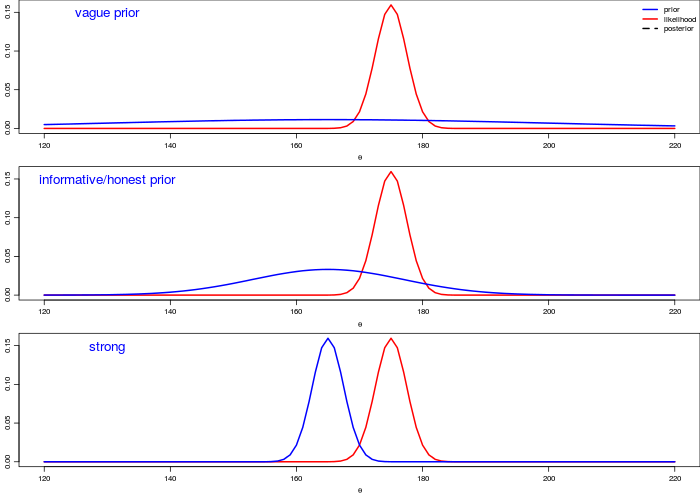
\includegraphics[width=.9\linewidth]{priors1.png}

Competing information: priors vs. likelihood
\end{frame}
\begin{frame}[label=sec-21]{Posterior $\propto$ Likelihood x Prior}
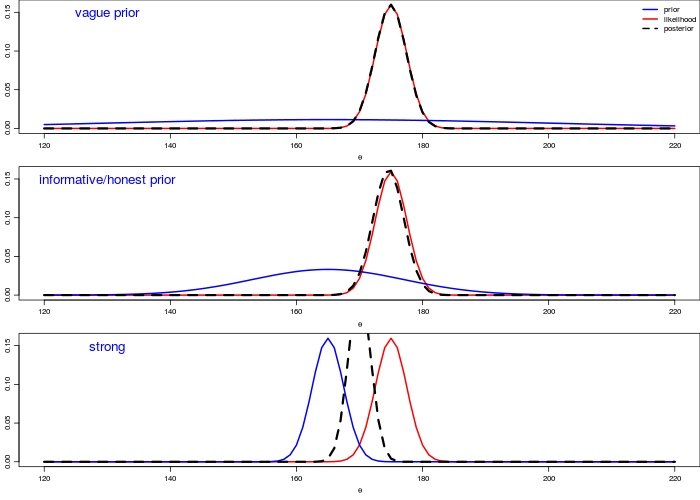
\includegraphics[width=.9\linewidth]{priors2.png}

Competing information: priors vs. likelihood
\end{frame}

\begin{frame}[label=sec-22]{Types of Priors}
\begin{block}{non-informative priors}
\begin{itemize}
\item desire Posterior estimates similar to MLE
\item deliberately ignore prior knowledge
\item Jeffrey's priors
\end{itemize}
\end{block}

\begin{block}{'Subjective Bayes'}
\begin{itemize}
\item honest representation of your actual knowledge
\item inference: how the data (via likelihood) updates Prior -> Posterior
\end{itemize}
\end{block}

\begin{block}{Strong Priors}
\begin{itemize}
\item computational reasons
\item 'fixing' parameters to a certain value
\item non-identifiability of parameter
\end{itemize}
\end{block}
\end{frame}

\begin{frame}[label=sec-23]{Types of Priors}
\begin{block}{Know the distributions and their parameters}
\begin{figure}[htb]
\centering
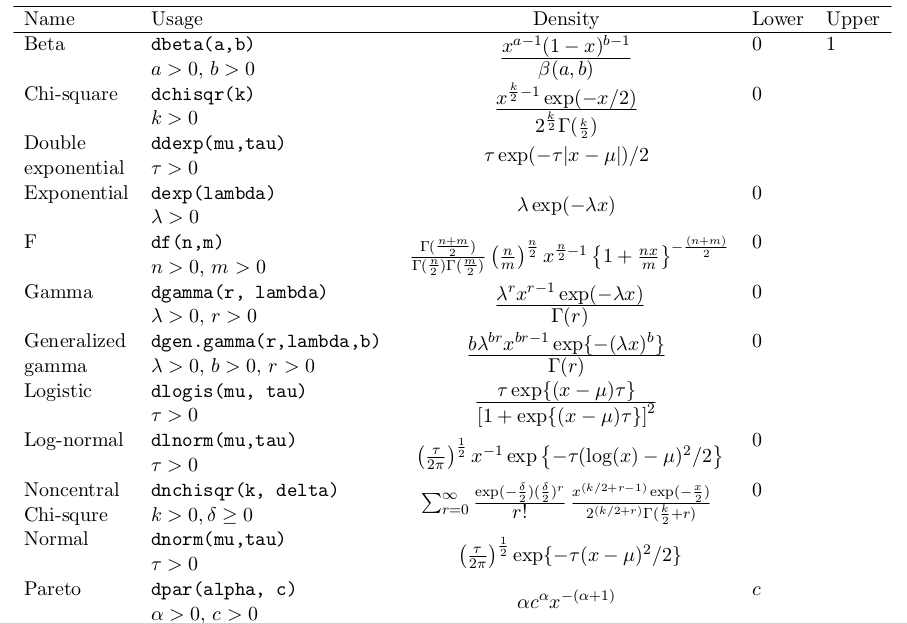
\includegraphics[width=.9\linewidth]{//home/rob/Documents/school/Murdoch/MURUG/tutorials/bayesian/distr.jpg}
\caption{\label{fig:foo}rjags Plummer 2015}
\end{figure}
\end{block}
\end{frame}

\begin{frame}[fragile,label=sec-24]{Types of Priors}
 \begin{block}{Know the distributions and their parameters}
Familiarize yourself with distributions: plot it, calculate some statistics
\begin{itemize}
\item Beta distribution example
\end{itemize}
\begin{verbatim}
r <- rbeta(10000, 0.5, 0.5)
\end{verbatim}

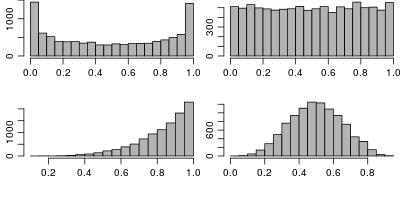
\includegraphics[width=.9\linewidth]{beta.jpg}
\end{block}
\end{frame}
\begin{frame}[label=sec-25]{Bayesian Analysis Example}
Time to open up R and JAGS
\begin{block}{'JAGS: Just Another Gibbs Sampler'}
Uses BUGS-like syntax (similar to OpenBUGS, WinBUGS)
\begin{itemize}
\item rjags Package: R friendly JAGS interface
\item easy easy easy Bayesian inference
\end{itemize}
Don't worry about 'samplers': JAGS does the hard work
\begin{itemize}
\item specify \textbf{likelihood} (how the data arose) and the \textbf{priors}
\end{itemize}
\end{block}
\end{frame}

\begin{frame}[fragile,label=sec-26]{Bayesian Analysis Example}
 example model: height of 20 Australian

\color{blue}
\begin{verbatim}
y <- c(183.46, 182.32, 178.31, 181.36, 165.12, 
185.68, 170.47, 178.11, 174.86, 182.03, 180.09, 
172.88, 177.94, 177.26, 182.58, 171, 173.74, 177.78, 
180.02, 163.05)
\end{verbatim}

\color{black}
\begin{itemize}
\item lets estimate the mean height (mu) and the dispersion (sigma)
\end{itemize}
\begin{small}
JAGS we estimate the 'precision' (tau): $\tau=\frac{1}{\sigma^2}$
\end{small}
\begin{figure}[htb]
\centering
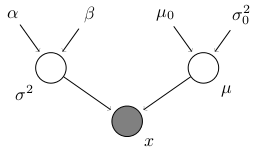
\includegraphics[width=0.4\textwidth]{//home/rob/Documents/school/Murdoch/MURUG/tutorials/bayesian/graph.png}
\caption{Prof Mike Jordan lecture notes}
\end{figure}
\end{frame}
\begin{frame}[label=sec-27]{Bayesian Analysis Example 1}
\begin{itemize}
\item open up R angs rjags
\item download and open the R file:
\end{itemize}
\end{frame}

\begin{frame}[fragile,label=sec-28]{Bayesian Analysis Example 1}
 Jags model syntax: specify priors and likelihood
\begin{verbatim}
model.txt<-'model{
 # Normal priors on mean height
 mu0 <- 100 
 sigma0 <- 35
 tau0 <- pow(sigma0,-2)
 mu ~ dnorm(mu0,tau0) 
 # Gamma prior on precision
 alpha0 <- 0.1
 beta0 <- 0.1
 tau ~ dgamma(alpha0,beta0)
 # Likelihood: how the data arose
 for(i in 1:length(y)){
   y[i] ~ dnorm(mu,tau) T(0,) # truncated normal
 }
 sigma <- pow(tau,-0.5)
}'
\end{verbatim}
\end{frame}

\begin{frame}[label=sec-29]{Sample-based inference}
\begin{block}{Posteriors}
often no 'analytical' solution to $P(\theta\vert Y)$
\end{block}

\begin{block}{Solution: Sampling}
\begin{itemize}
\item it is a Probability Distribution!!!
\item find a way to "sample" from posterior.
\item with enough samples: mean(samples) = Posterior Expectation
\end{itemize}
\end{block}

\begin{block}{Sampling Algorithms}
MCMC; Gibbs Sampling; Metropolis-Hastings; Slice-Sampling; Importance Sampling; "Conjugate Priors"; conditional probability
\begin{itemize}
\item all (sub)algorithms or concepts or techniques to help sample a posterior
\end{itemize}
\end{block}
\end{frame}
\begin{frame}[label=sec-30]{Approximate the joint-posterior distribution"}
\begin{block}{example: estimate mean and variance of $\theta$}
$\theta_{\text{true}}=3.44$; $\text{Var}(\theta)_{\text{true}}=4.89$
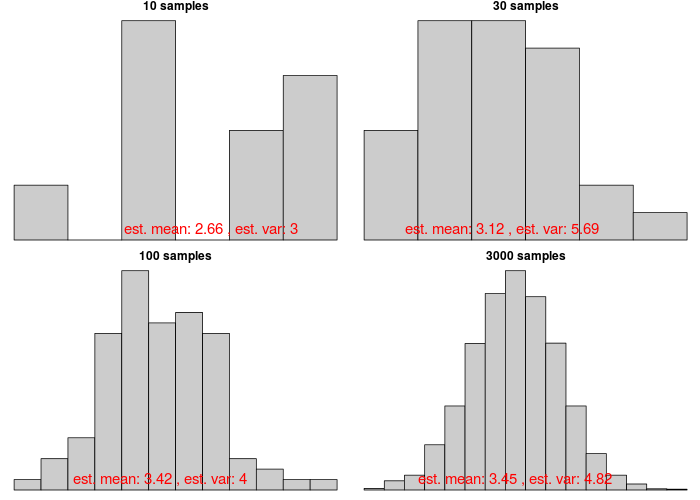
\includegraphics[width=.9\linewidth]{samples1.png}
\end{block}
\end{frame}
\begin{frame}[label=sec-31]{Gibbs Sampling}
break-down joint posterior into (simpler) conditional distributions
\begin{itemize}
\item difficult: sampling $P(\beta_0,\beta_1,\beta_2,\sigma^2\vert Y)$
\item easy: sampling $P(\beta_0,\beta_1,\beta_2,\vert\sigma^2, Y)$ then $P(\sigma^2\vert\beta_0,\beta_1,\beta_2,Y)$ then repeat
\end{itemize}
approximates the joint posterior
\begin{block}{algorithm}
\begin{itemize}
\item initialize: $\beta_0^{(0)},\beta_1^{(0)},\beta_2^{(0)},\sigma^{2(0)}$
\end{itemize}
\begin{equation}
\begin{aligned}
\{\beta_0^{(1)},\beta_1^{(1)},\beta_2^{(1)}\} &\ \sim P(\beta \vert \sigma^{2(0)},Y) \\
\sigma^{2(1)} &\ \sim P(\sigma^2 \vert \beta_0^{(1)},\beta_1^{(1)},\beta_2^{(1)},Y) \\
\{\beta_0^{(2)},\beta_1^{(2)},\beta_2^{(2)}\} &\ \sim P(\beta \vert \sigma^{2(1)},Y) \\
\sigma^{2(2)} &\ \sim P(\sigma^2 \vert \beta_0^{(2)},\beta_1^{(2)},\beta_2^{(2)},Y)
\end{aligned}
\end{equation}
\begin{itemize}
\item repeat 1000's or 1000000 's times
\end{itemize}
\end{block}
\end{frame}
\begin{frame}[label=sec-32]{BUGS to the rescue}
Previously, Bayesian analysis demanded custom-coding MCMC algorithms
\begin{block}{WinBUGS \& OpenBUGS \& JAGS}
automatically use appropriate sampling techniques; so we don't have to worry
\end{block}

\begin{block}{BUT you must: Monitor the MCMC!}
\begin{itemize}
\item give reasonable \textbf{initial values}
\item ensure \textbf{convergence}: no trend; independent chains give same answer
\item ensure adequate \textbf{mixing}: independent samples
\end{itemize}
\end{block}
\end{frame}

\begin{frame}[label=sec-33]{MCMC: Good mixing}
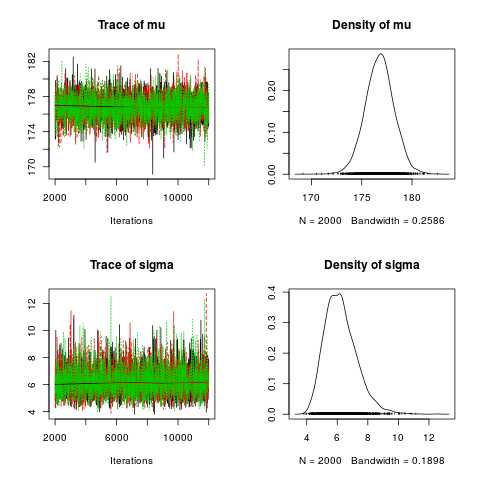
\includegraphics[width=.9\linewidth]{//home/rob/Documents/school/Murdoch/MURUG/tutorials/bayesian/mcmc_goodmix.jpg}
\end{frame}

\begin{frame}[label=sec-34]{MCMC: Poor convergence}
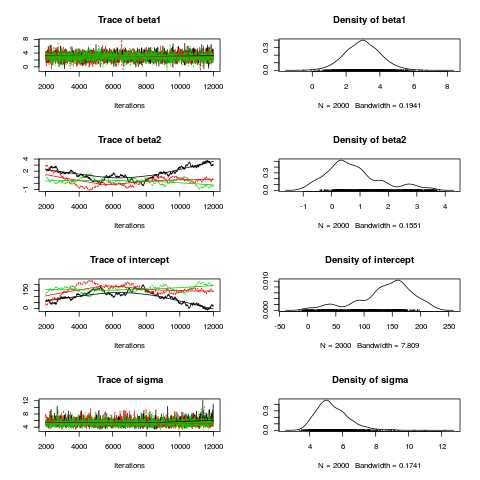
\includegraphics[width=.9\linewidth]{//home/rob/Documents/school/Murdoch/MURUG/tutorials/bayesian/mcmc_goodbad.jpg}
\end{frame}

\begin{frame}[label=sec-35]{MCMC}
\begin{block}{MCMC parameters in JAGS}
\begin{itemize}
\item n.chains: num. of MCMC chains; more is better
\item n.adapt: discard first samples; let algorithm 'adapt'
\item n.burn: discard extra samples; allow algorithm to reach startionary distribution
\item n.iter: total number of sample; more is better
\item thin: take every $k^{th}$ iteration for a sample; decorrelates one sample from the next; higher is better
\item total samples: number of samples to approximate your Posterior; target at least 2000 to 5000
\end{itemize}
\end{block}
\end{frame}

\begin{frame}[label=sec-36]{MCMC: what to do with bad mixing}
\begin{itemize}
\item run longer chains
\item ensure long enough adaption phase
\item misspecified priors
\item bad initial values?
\end{itemize}
\end{frame}

\begin{frame}[label=sec-37]{Advantages of Bayesian Inference}
\begin{itemize}
\item inference statesments: easy to understand (only Bayesians can make probabilistic statements about $\theta$)
\item small sample sizes: exact inference
\item missing data: very easy to impute
\item integrate other information, or calculate 'derived parameters'
\end{itemize}
\begin{block}{Hierarchical Bayesian}
\begin{itemize}
\item model dependences (space \& time)
\item "random-effects" models
\item "model-selection" / "model-multi inference" (AIC, Lasso, etc., are just types of Bayesian models)
\item shrinkage: deflate influence of outlier values
\end{itemize}
\end{block}
\end{frame}
\begin{frame}[label=sec-38]{Where to go from here?}
\begin{block}{some Bayesian learning resources}
\begin{itemize}
\item learn about prior distributions!
\item great R package for learning the fundamentals of Gibbs sampling, MCMC, conditional probability, etc.
\end{itemize}
\verb!LearnBayes: Functions for Learning Bayesian Inference! See the Vignettes. \url{https://cran.r-project.org/web/packages/LearnBayes/index.html}
\begin{itemize}
\item OpenBUGS examples: read and run yourself
\end{itemize}
\url{http://www.openbugs.net/w/Examples}
\begin{itemize}
\item Textbook: WinBUGs for Ecologists, Marc Kery
\item Blog: Andrew Gelman: \url{http://andrewgelman.com/}
\end{itemize}
\end{block}

\begin{block}{Frequentism}
\begin{itemize}
\item Excellent and accessible video lecture by Michael Jordan
\end{itemize}
\url{http://videolectures.net/mlss09uk_jordan_bfway/}
\begin{itemize}
\item 
\end{itemize}
\end{block}
\end{frame}
% Emacs 24.3.1 (Org mode 8.2.5g)
\end{document}
